\mychapter{Resultat}
\label{chap:resultat}
Notera att tiden som visas i tabellerna är i sekunder och är ett medelvärde av 25 enskilda
krypteringsomgångar för varje nyckel och varje körläge. Det råa data värdena från hela undersökningen
går att se i bilaga \ref{app:raw-data-mode-picture-test}, \ref{app:raw-data-keylength} \& \ref{app:raw-data-mode}.

\section{Nyckellängds Test}
\label{sec:nyckellangd}

\begin{table}[H]
    \centering
    \begin{tabular}{ ||c|c|c|| }
      \hline
      \multicolumn{3}{|c|}{\bfseries{Resultat Tid (s)}} \\
      \hline
      \bfseries{ECB - 128bit} & \bfseries{ECB - 192bit} & \bfseries{ECB - 256bit} \\
      \hline
      21.05752382799983 & 25.014501572000153 & 29.177583716000083 \\
      \hline
    \end{tabular}
\end{table}

\section{Körläges Test}
\label{sec:korlages}

\begin{table}[H]
    \centering
    \begin{tabular}{ ||c|c|c|| }
      \hline
      \multicolumn{3}{|c|}{\bfseries{Resultat Tid (s)}} \\
      \hline
      \bfseries{ECB - 128bit} & \bfseries{CBC - 128bit} & \bfseries{OFB - 128bit} \\
      \hline
      20.82165230000013 & 20.885069635999972 & 20.89562146799988 \\
      \hline
    \end{tabular}
\end{table}

\section{Krypterings Test}
\label{sec:krypterings-test}

\begin{figure}[H]
    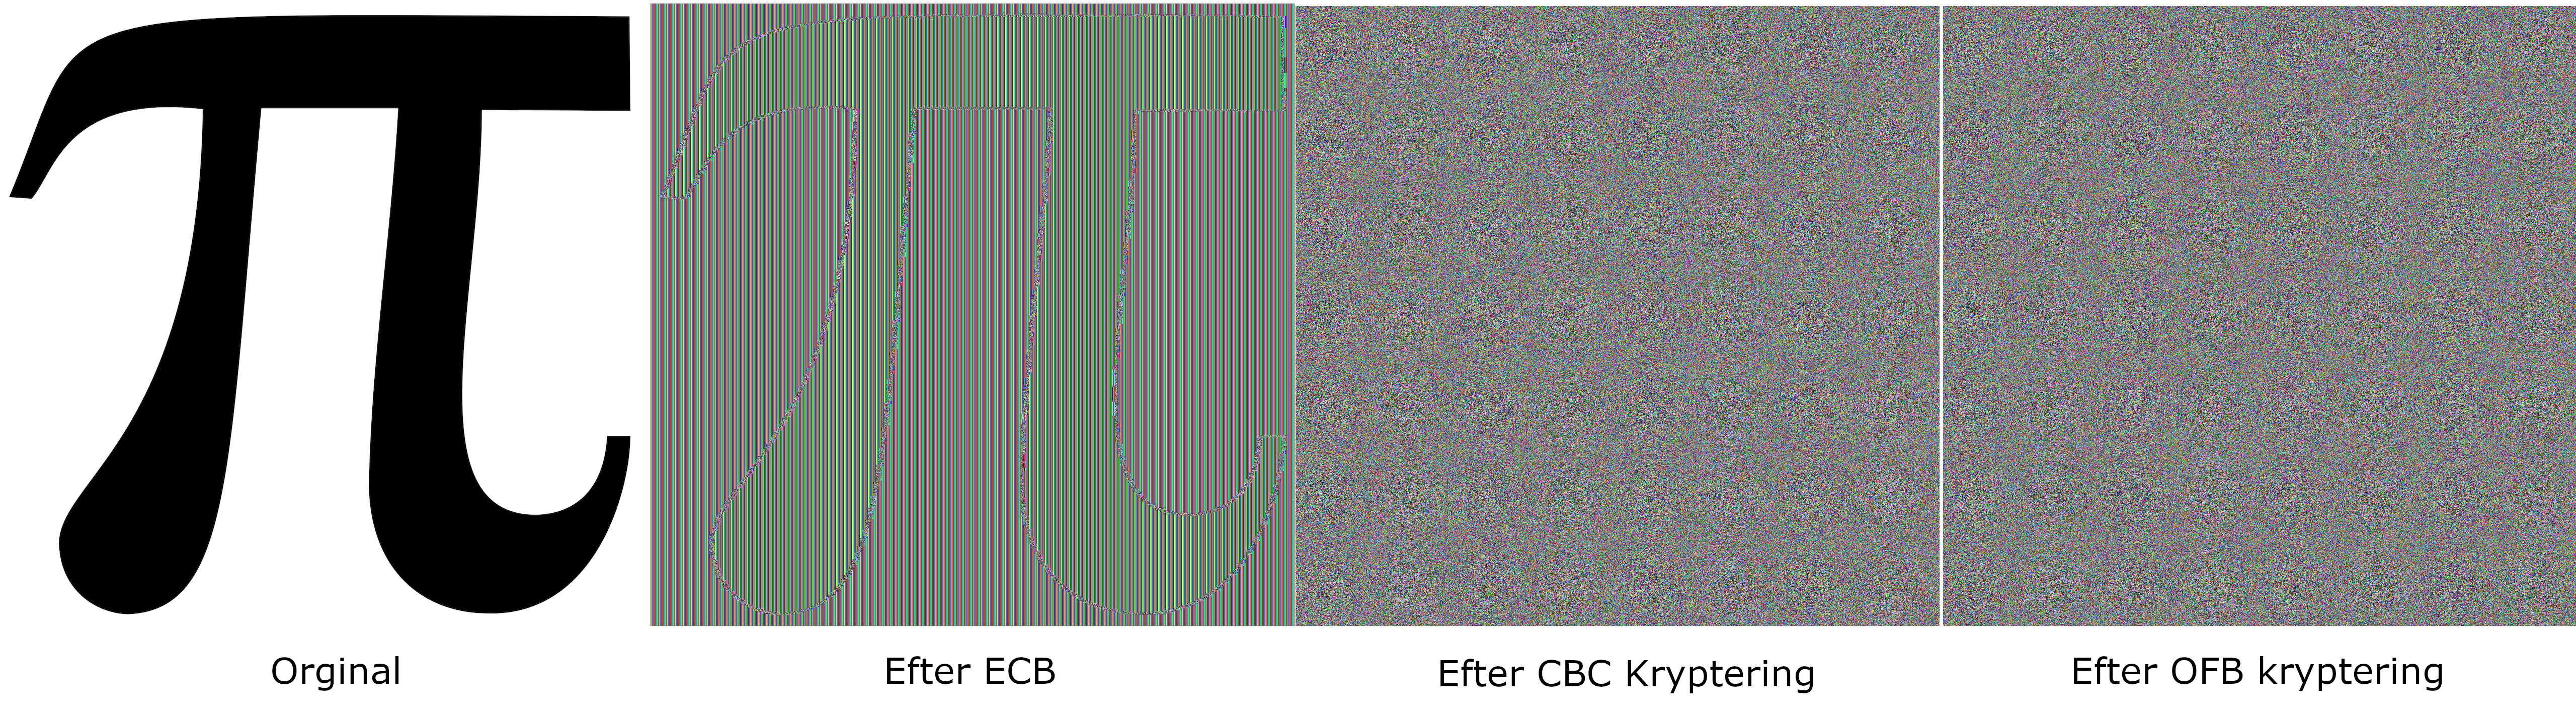
\includegraphics[width=\textwidth]{summarie-tp-background.png}
    \caption{\acrshort{aes} krypterings test (\acrshort{ecb}, \acrshort{cbc}, \acrshort{ofb})}
    \label{fig:aes-krypterings-test}
\end{figure}
